%!TEX root = ../Documentazione.tex
%%--------------------------------------------------------------------------
%% INTERFACCIA UTENTE
%%--------------------------------------------------------------------------



\chapter{User Interface}
\label{chap:ui}

	\section{Master-Details layout}
	As decided in the Design Document, the main screen of the application, containing the list of alarms, is presented in different ways depending on the screen size of the device: in particular, on large screens the list and the details of alarms are shown one next to each other. To get this kind of layout were exploited {\tt Fragmen}, UI components which have the particularity of being able to be reused in multiple {\tt Activity} maintaining their application logic. The classes used to achieve this behavior are:

		\begin{itemize}

			\item MainActivity

			\item AlarmDetailActiviy

			\item AlarmListFragment

			\item AlarmDetailFragment

		\end{itemize}

	It's has been also created a file {\tt refs.xml} in the folder res/values-sw600dp:

		\begin{lstlisting}
<resources>
    <item type="layout" name="activity_alarm_list">@layout/activity_alarm_twopane</item>
</resources>
		\end{lstlisting}
	along with files \texttt{activity\_alarm\_list.xml} and \texttt{activity\_alarm\_twopane.xml} in the folder res/layout.
	Starting {\tt MainActivity} and executing:

		\begin{lstlisting}
inflater.inflate(R.layout.activity_alarm_list, container, false);
		\end{lstlisting}

	Android will know which of the two layouts to choose, thanks to the alias contained in {\tt refs.xm}, depending on the size of the display. In fact the system will choose the resources contained in folders with suffix ``-sw600dp'' when the width of the display will be greater than 600 dp. 
	In this way it is possible to recognize whether the code is run on a tablet or a smartphone then choosing to put side by side {\tt 
	AlarmListFragment} and {\tt AlarmDetailFragment} in the first case or only {\tt AlarmListFragment} in the latter.

		\begin{figure}[h!]
		  \centering
		    \centering{%
		      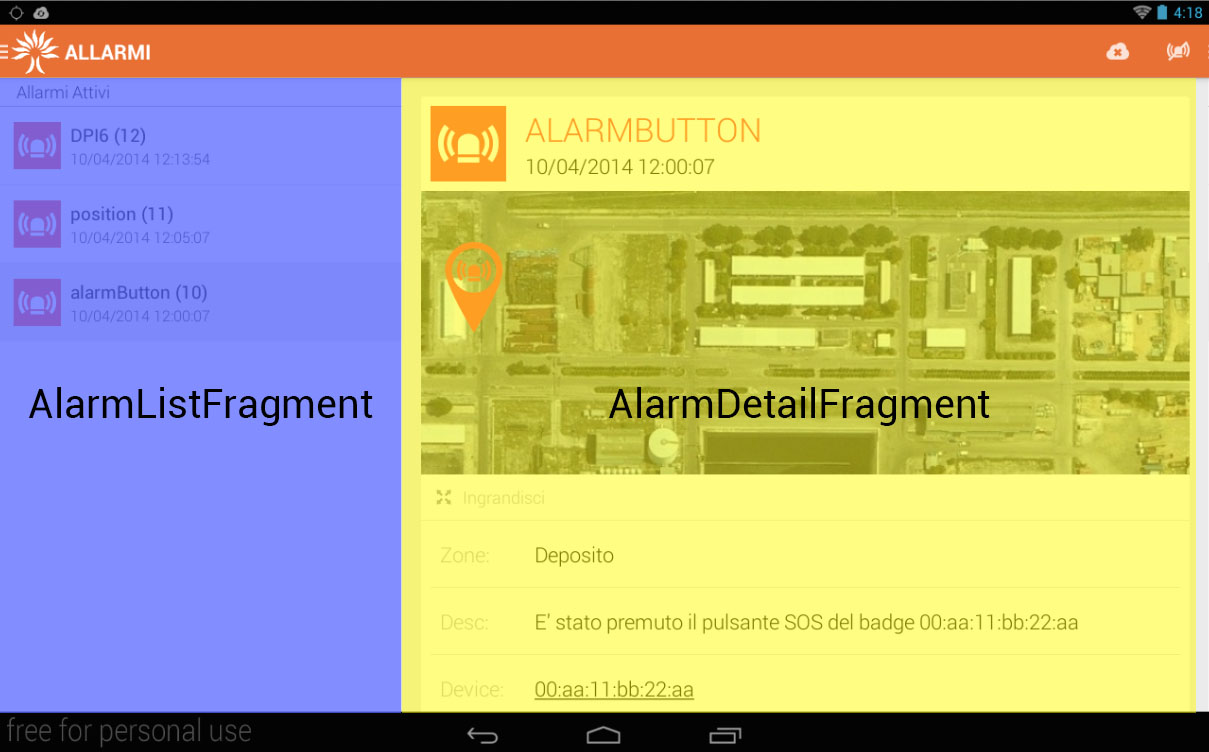
\includegraphics[width=1\textwidth]{master_detail_tablet.jpg}}
		  \caption{Master-Details layout - Tablet}
		\end{figure}

		\begin{figure}[h!]
		  \centering
		    \centering{%
		      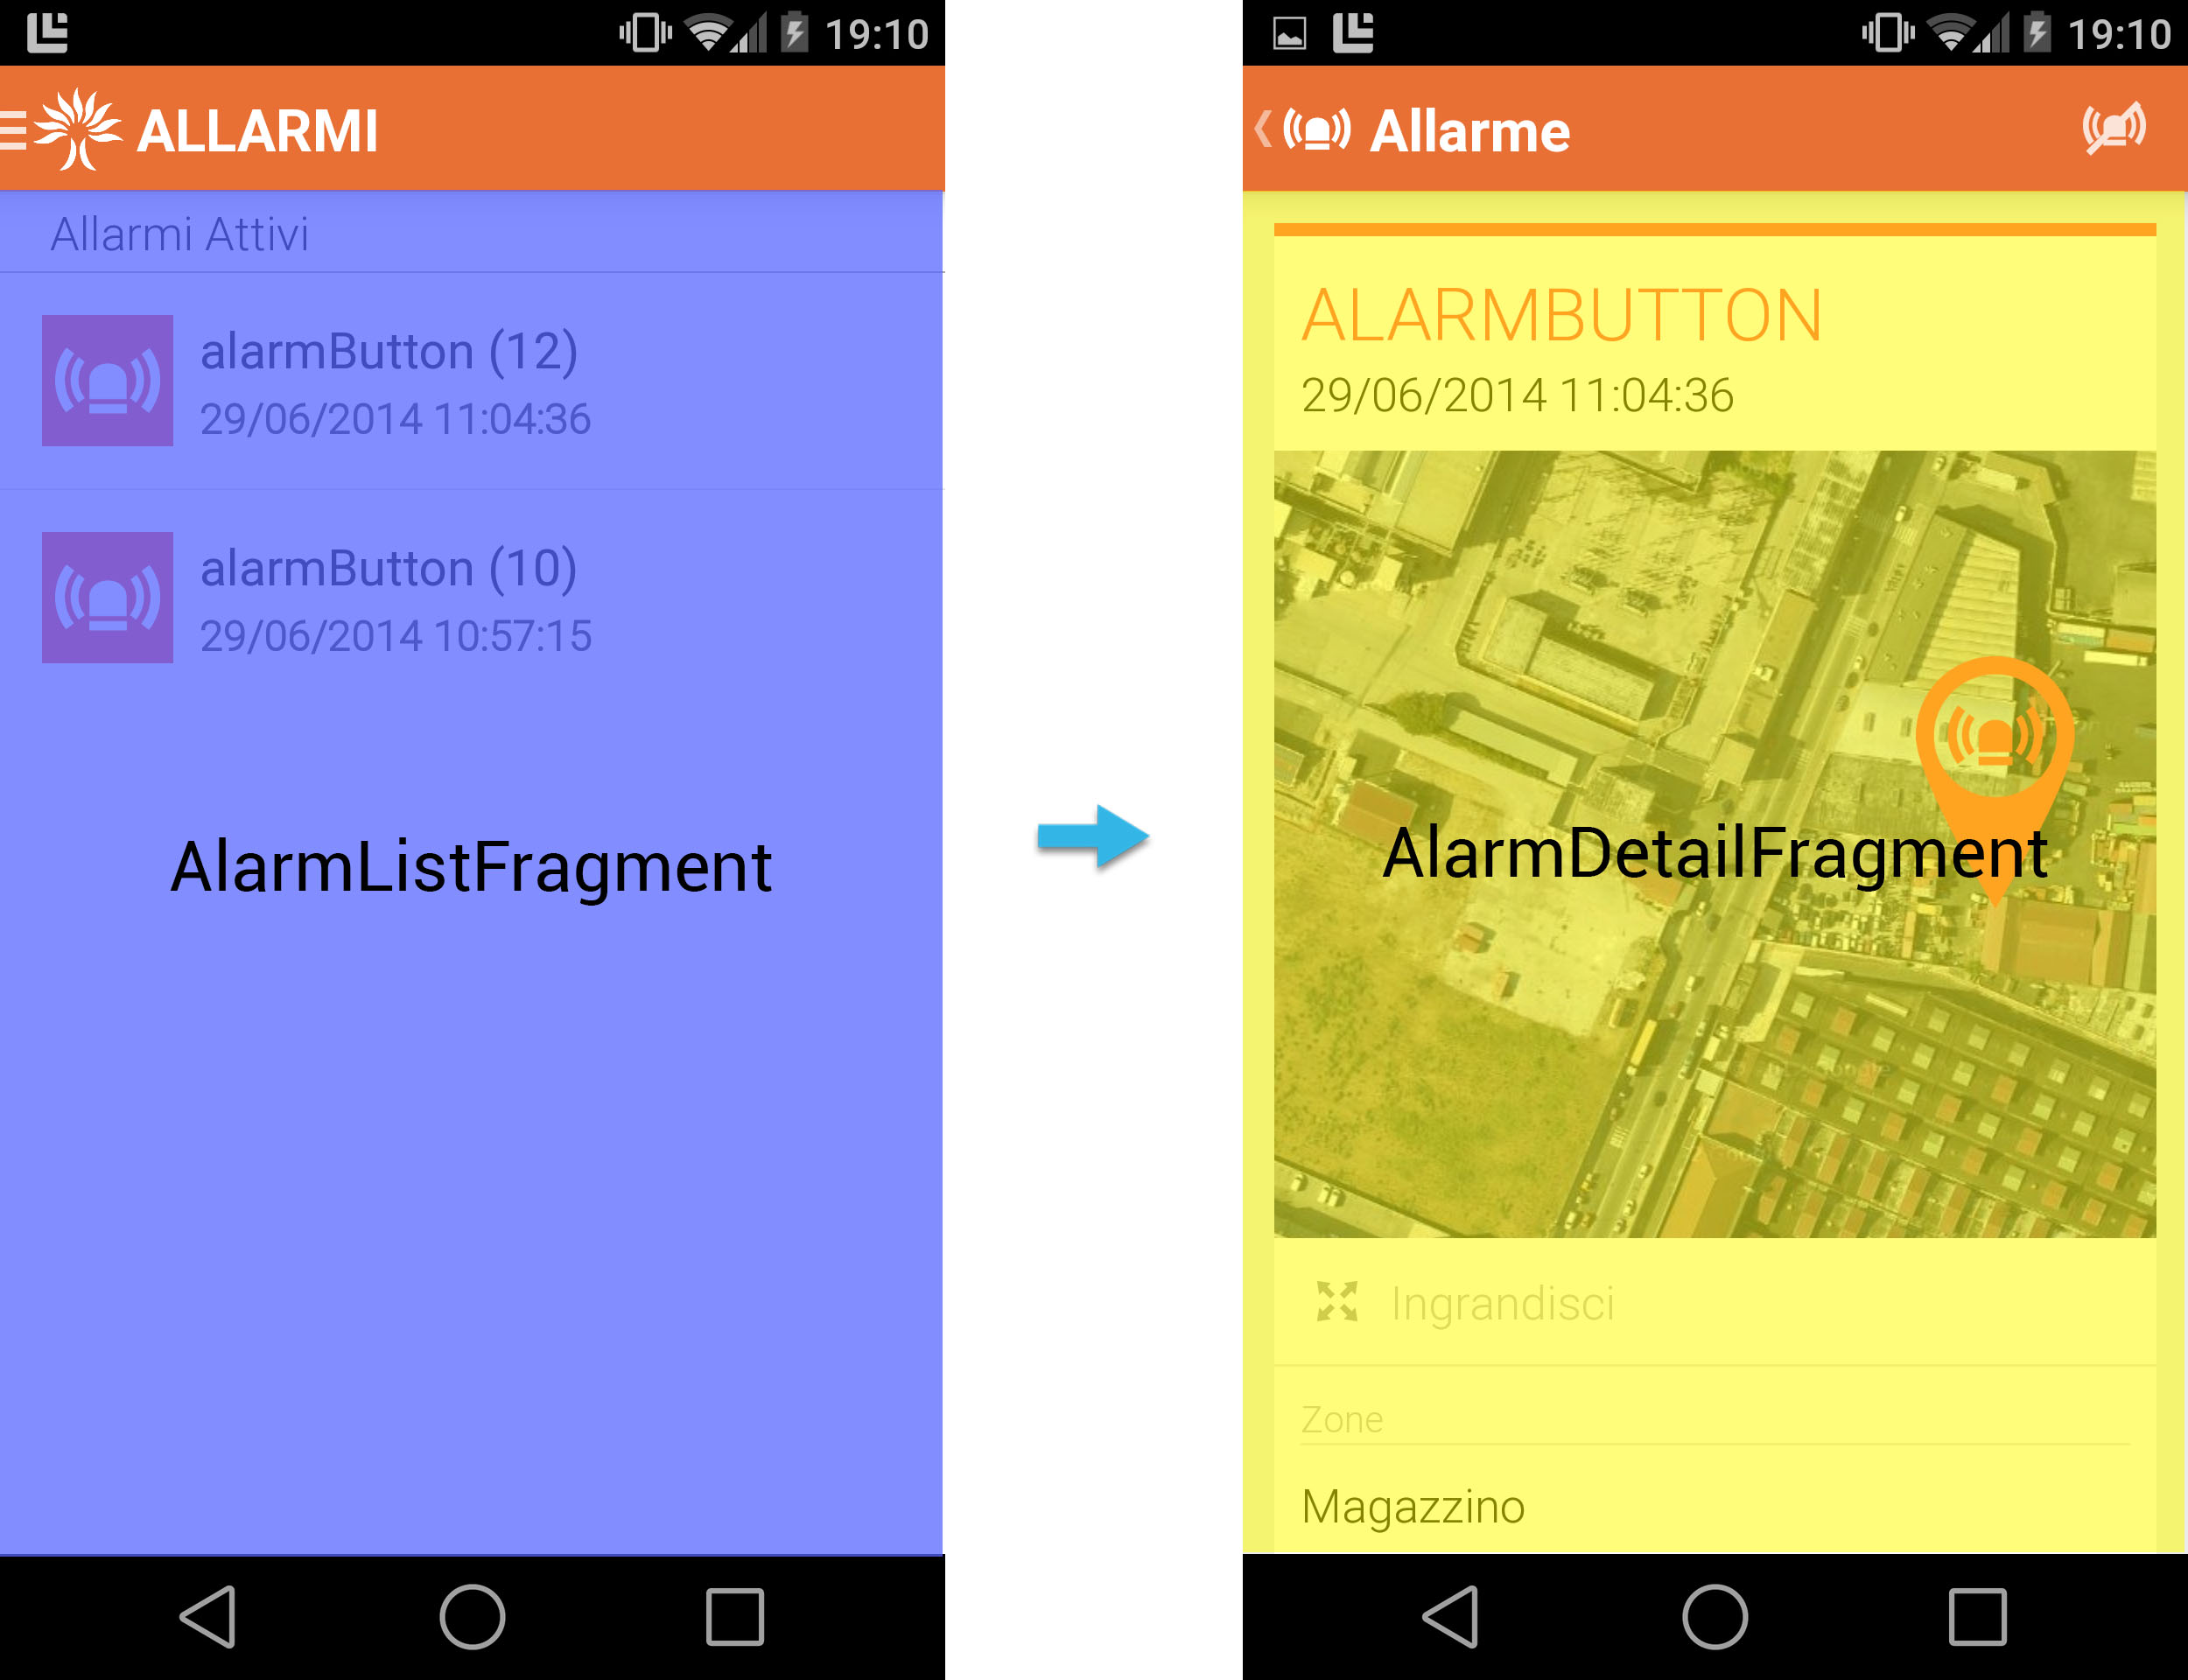
\includegraphics[width=1\textwidth]{master_detail_phone.jpg}}
		  \caption{Master-Details layout - Phone}
		\end{figure}


	\newpage
	\section{AlarmDetailActivity}
	This {\tt Activity} is launched thanks to an {\tt Intent} which contains an extra parameter that indicates the id of the alarm that will displayed:

		\begin{lstlisting}
    Intent detailIntent = new Intent(mActivity, AlarmDetailActivity.class);
    detailIntent.putExtra(AlarmDetailFragment.ARG_ITEM_ID, id);
		\end{lstlisting}




	\section{NotificationsManager}
	he management of notifications has been enclosed in the class {\tt NotificationsManager}. The class has two {\tt Notifications}:

		\begin{description}

			\item[NOTIF\_ONGOING\_SERVICE] Notification permanently associated with the background service as described in section \ref{startForeground()}; the text of the notification is updated with the appropriate methods. Tapping it launches the app.

			\item[NOTIF\_ONGOING\_ALARMS] Notification displayed permanently until there are new alarms not yet readed. Tapping it launches the alarm list.

		\end{description}




